\documentclass[a4paper,12pt]{article}
\usepackage[francais]{babel}
\usepackage[utf8]{inputenc}
\usepackage[T1]{fontenc}
\usepackage{graphicx}
\usepackage{geometry}
\usepackage{amsmath}
\usepackage{float}
\usepackage{listings}
\usepackage{xcolor}
\usepackage{hyperref}
\usepackage{rotating}

\setcounter{secnumdepth}{0}
\hypersetup{colorlinks=true, linkcolor=black}
\geometry{margin=1in}

\definecolor{codegreen}{rgb}{0,0.5,0.07}
\definecolor{codeblue}{rgb}{0.05,0,1.0}
\definecolor{codepurple}{rgb}{0.65,0.35,0.96}
\lstdefinestyle{mystyle}{
    commentstyle=\color{codegreen},
    keywordstyle=\color{codeblue},
    stringstyle=\color{codepurple},
    basicstyle=\ttfamily\normalsize,
    breakatwhitespace=true,
    breaklines=true,
    frame=lines,
}
\lstset{style=mystyle}

\begin{document}

\selectlanguage{french}

\begin{titlepage}
    \begin{center}
        % Logo de l'école en en-tête
        
\includegraphics[width=5cm]{./img/uqac.png}\\[1cm]
        
        % Titre principal
        \vspace*{1cm} % Ajuster pour centrer verticalement
        {\Huge \textbf{Interaction Humain-Robot : Devoir 2}\\[0.5cm]}

        % Image de couverture (centrée en dessous du logo)
        \vspace*{1cm}
        
\includegraphics[width=0.7\textwidth]{./img/image_IHR.png}\\[1cm]

        \vspace{4.5cm}
        \begin{tabular*}{1\linewidth}{@{\extracolsep{\fill}}l c r}
            {\large Constance ALOYAU} &  & {\large ALOC25530200} \\
            {\large Erwan MAWART} & {\large 16 novembre 2024} & {\large MAWE14050200} \\
            {\large Benjamin PELLIEUX} &  & {\large PELB28120100} \\
        \end{tabular*}
        
        \vfill
    \end{center}
\end{titlepage}

\tableofcontents
\newpage

\section{Introduction}

    Les vibrations dans un mécanisme robotique manipulé par un opérateur humain peuvent significativement compromettre la précision et la qualité de la tâche effectuée. Lorsque l’opérateur applique une force via une poignée équipée d’un capteur, des vibrations non désirées peuvent survenir, surtout lorsque l'opérateur ajuste la rigidité de son bras. Ces vibrations perturbent non seulement la performance mais réduisent aussi le confort de l’utilisateur.

    Dans le cadre de ce projet, nous cherchons à modéliser et analyser l'impact perceptuel de ces vibrations en interaction humain-robot (IHR). Notre approche implique le développement d'un observateur de vibrations capable de détecter et segmenter les parties du signal problématiques, permettant ainsi un ajustement dynamique d’un contrôleur proportionnel en fonction de l'indice de vibration mesuré. L’objectif est de minimiser ces vibrations, tout en tenant compte de l’expérience ressentie par l’opérateur.

    Ce rapport aborde plusieurs aspects de la conception et de la simulation du modèle du mécanisme, incluant la formulation des équations d’état du système, l’implémentation d’un critère de stabilité basé sur le critère de Routh-Hurwitz, ainsi que la configuration de la boucle de contrôle pour limiter les vibrations. Nous explorons également la détection autonome des caractéristiques vibratoires à travers une simulation pour tester l'efficacité de notre modèle dans des scénarios variés.

\newpage
\section{Énoncé 1 : Conception du modèle du mécanisme}
\subsection{Question 1.1}
\begin{figure}[h!]
    \centering
    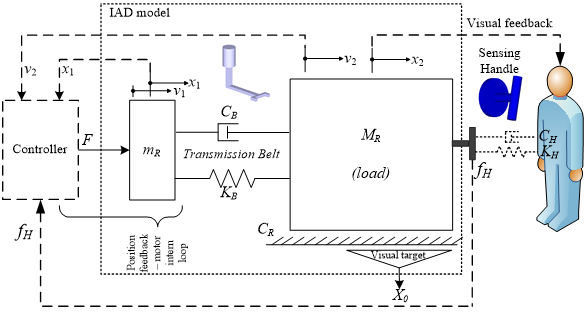
\includegraphics[width=14cm]{./img/modele_humain-meca_robotique.png}
    \caption{Modèle du mécanisme robotique et de l'humain \label{fig:ModelMecaRobotHumain}}
\end{figure}

La \hyperref[fig:ModelMecaRobotHumain]{\autoref{fig:ModelMecaRobotHumain}} présente le mécanisme robotique que nous allons utiliser, où :
\begin{itemize}
    \item[$\bullet$] $M_R$ : masse de la charge \textit{[kg]}.
    \item[$\bullet$] $m_R$ : masse du système \textit{[kg]}.
    \item[$\bullet$] $K_B$ : constante de raideur des courroies \textit{[N/m]}.
    \item[$\bullet$] $C_B$ : coefficient d'amortissement des courroies \textit{[$N\cdot s/m$]}.
    \item[$\bullet$] $K_H$ : coefficient de raideur de l'humain\textit{[N/m]}.
    \item[$\bullet$] $C_H$ : coefficient d'amortissement de l'humain \textit{[$N\cdot s/m$]}.
    \item[$\bullet$] $C_R$ : coefficient de frottement \textit{[$N\cdot s/m$]}.
    \item[$\bullet$] $F$ : Force commandée par le système \textit{[N]}.
    \item[$\bullet$] $f_H$ : Force appliquée par l'humain \textit{[N]}.
    \item[$\bullet$] $x_1$ : position des moteurs \textit{[m]}.
    \item[$\bullet$] $x_2$ : position de la charge \textit{[m]}.
    \item[$\bullet$] $v_1$ : vitesse des moteurs \textit{[m/s]}, la dérivée de la position ($v_1 = \dot{x_1}$).
    \item[$\bullet$] $v_2$ : vitesse de la charge \textit{[m/s]}, la dérivée de la position ($v_2 = \dot{x_2}$).
\end{itemize}

Ainsi, on déduit les variables d'états ci-dessous.
\[
    X =
    \begin{bmatrix}
        x_1 \\
        x_2 \\
        v_1 \\
        v_2
    \end{bmatrix}
    =
    \begin{bmatrix}
        x_1 \\
        x_2 \\
        \dot{x_1} \\
        \dot{x_2}
    \end{bmatrix}
\]

En effectuant la somme des forces appliquées sur chaque masse, on obtient le système suivant.
\[
    \begin{cases}
        \sum F_{ext/m_R} = m_R\ddot{x_1} \\
        \sum F_{ext/M_R} = M_R\ddot{x_2} \\
    \end{cases}
    \Leftrightarrow
    \begin{cases}
        m_R\ddot{x_1} = F - K_B x_1 + K_B x_2 - C_B \dot{x_1} + C_B\dot{x_2} \\
        M_R\ddot{x_2} = K_B x_1 - K_B x_2 + C_B \dot{x_1} - C_B\dot{x_2} - C_R \dot{x_2} \\
    \end{cases}
\]

\begin{equation}
    \\ \Leftrightarrow
    \begin{cases}
        \ddot{x_1} = \frac{F - K_B x_1 + K_B x_2 - C_B \dot{x_1} + C_B \dot{x_2}}{m_R} \\
        \ddot{x_2} = \frac{K_B x_1 - K_B x_2 + C_B \dot{x_1} - C_B \dot{x_2} - C_R \dot{x_2}}{M_R}
    \end{cases}
    \label{eq:SommeDesForces}
\end{equation}

Grâce à celle-ci, on construit les deux équations de fonctionnement du système :

\begin{equation}
    \dot{X}=AX+BU
    \Leftrightarrow
    \begin{bmatrix}
        \dot{x_1}\\
        \dot{x_2}\\
        \ddot{x_1}\\
        \ddot{x_2}
    \end{bmatrix}
    =
    \begin{bmatrix}
        0 & 0 & 1 & 0\\
        0 & 0 & 0 & 1\\
        \frac{-K_B}{m_R} & \frac{K_B}{m_R} & \frac{-C_B}{m_R} & \frac{C_B}{m_R}\\
        \frac{K_B}{M_R} & \frac{-K_B}{M_R} & \frac{C_B}{M_R} & \frac{-(C_B+C_R)}{M_R}\\
    \end{bmatrix}
    \begin{bmatrix}
        x_1\\
        x_2\\
        \dot{x_1}\\
        \dot{x_2}
    \end{bmatrix}
    +
    \begin{bmatrix}
        0\\
        0\\
        \frac{1}{m_R}\\
        0
    \end{bmatrix}
    \cdot F
    \label{eq:VarEtatXDot}
\end{equation}

\begin{equation}
    Y=CX+DU
    \Leftrightarrow
    Y=CX
    \Leftrightarrow
    \begin{bmatrix}
        x_2\\
        \dot{x_1}
    \end{bmatrix}
    =
    \begin{bmatrix}
        0 & 1 & 0 & 0\\
        0 & 0 & 1 & 0
    \end{bmatrix}
    \begin{bmatrix}
        x_1\\
        x_2\\
        \dot{x_1}\\
        \dot{x_2}
    \end{bmatrix}\\
    \label{eq:VarEtatY}
\end{equation}

L'\autoref{eq:VarEtatY} présente la sortie du système. Dans notre cas, on utilise $x_2$ (la position de la charge) et $v_1$ (la vitesse des moteurs) afin d'asservir notre système. Où $x_2$ permet à l'humain de corriger la trajectoire de la charge et $v_1$ d'asservir les moteurs.


\subsection{Question 1.2}
Lors d'une étude précédente, nous nous penchions sur la détectection des vibrations générées par le système lorsque l'humain se régédifie. Pour cela, nous analysions la vitesse des moteurs pour en extraire des caractéristiques temporelles et/ou fréquentielles qui nous permettent de déterminer la présence des vibrations. \\

\begin{figure}[h!]
    \centering
    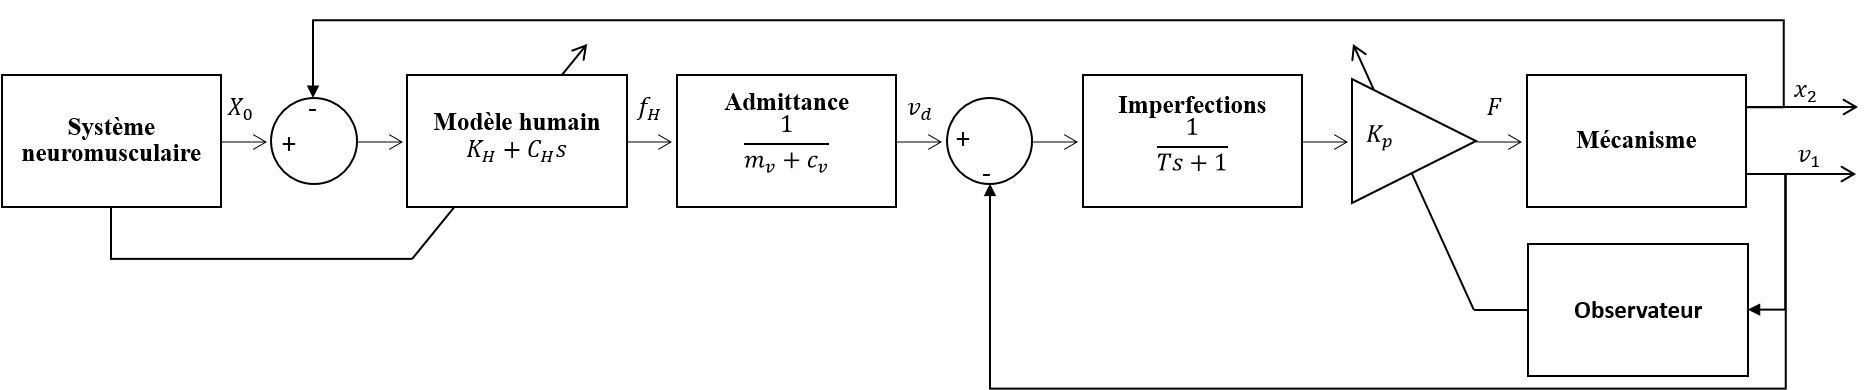
\includegraphics[width=16cm]{./img/SchemaBlocAvecObs.png}
    \caption{Commande des mécanisme robotique et humain avec observateur\label{fig:SchemaBlocAvecObs}}
\end{figure}

Afin de rendre le système autonome, il est donc nécessaire de rendre automatique cette recherche de caractéristiques. C'est pourquoi, comme le montre la \hyperref[fig:SchemaBlocAvecObs]{\autoref{fig:SchemaBlocAvecObs}}, on ajoute un observateur qui va influer sur la valeur du gain $K_p$, et donc, limiter les vibrations générées par le système.

Dans Simulink, on représentera ce bloc avec le programme suivant :
% à compléter



\newpage
\subsection{Question 1.3}
Le critère de Routh-Hurwitz est une méthode mathétique permettant déterminer rapidement la stabilité d'un système. Elle consiste à générer un tableau à partir des coefficients du dénominateur de la fonction de transfert tel que présenté au \autoref{tab:table_theo_critRH}. Une fois construit, on observe sa première colonne. Le nombre de changement de signe détermine la quantité de racines étant dans la partie astable du plan-s (c'est-à-dire dans la partie réel positive).

\begin{table}[ht]
    \centering
    \[
    \begin{array}{|c|c c c c|}
        \hline
        s^n & a_n & a_{n-2} & a_{n-4} & \dots \\
        \hline
        s^{n-1} & a_{n-1} & a_{n-3} & a_{n-5} & \dots \\
        \hline
        s^{n-2} & b_{n-1} & b_{n-3} & b_{n-5} & \dots \\
        \hline
        s^{n-3} & c_{n-1} & c_{n-3} & c_{n-5} & \dots \\
        \hline
        \vdots & \vdots & \vdots & \vdots & \vdots \\
        \hline
        s^0 & h_{n-1} & h_{n-3} & h_{n-5} & \dots \\
        \hline
    \end{array}
    \]
    \caption{Tableau théorique du critère de Routh-Hurwitz}
    \label{tab:table_theo_critRH}
\end{table}

Dans le \autoref{tab:table_theo_critRH}, on retrouve :
\begin{itemize}
    \item[$\bullet$] $a_{n-i}$, les coefficients du dénominateur.
    \item[$\bullet$] $b_{n-i}$, donnés par :
        $b_{n-i} = \frac{-1}{a_{n-1}}
        \begin{vmatrix}
            a_n & a_{n-i-1} \\
            a_{n-1} & a_{n-i-2}
        \end{vmatrix}
        = \frac{a_{n-1} a_{n-i-1} - a_n a_{n-i-2}}{a_{n-1}}$
    \item[$\bullet$] $c_{n-i}$, donnés par :
        $c_{n-i} = \frac{-1}{b_{n-1}}
        \begin{vmatrix}
            a_n & a_{n-i-2} \\
            b_{n-1} & b_{n-i-2}
        \end{vmatrix}
        = \frac{b_{n-1} a_{n-i-2} - a_n b_{n-i-2}}{b_{n-1}}$
    \item[$\bullet$] etc.
\end{itemize} 

On utilise cette méthode afin de déterminer la plage de valeurs des gain $K_p$ et $K_h$.
\subsubsection{Boucle de vitesse}
\begin{figure}[h!]
    \centering
    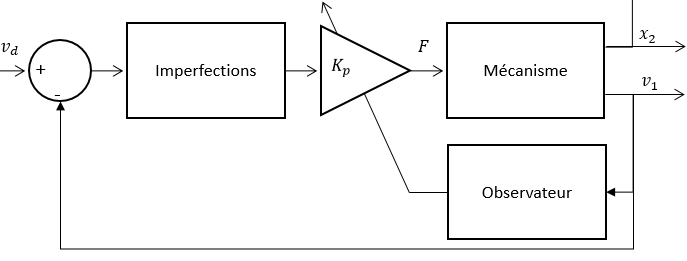
\includegraphics[width=8cm]{./img/cmd_meca_rob_hum_vit.png}
    \caption{Commande du mécanisme robotique}
    \label{fig:SchemaBlocMeca}
\end{figure}
Dans un premier temps, on étudie la plage du gain $K_p$ en se focalisant sur la boucle de vitesse présentée à la \hyperref[fig:SchemaBlocMeca]{\autoref{fig:SchemaBlocMeca}}. Afin de construire le critère de Routh-Hurwitz plus simplement, on utilise ce programme MATLAB : \\
\newpage
\begin{lstlisting}[language=Matlab]
    syms Kp Kh s

    % Extraction des coefficients du denominateur =====
    [~, Den] = numden(BoucleVitesse);
    [an, terms] = coeffs(Den, s);
    l_terms = length(terms);
    l = round(l_terms/2);

    % Creation du tableau =============================
    S = sym(zeros(l_terms, l)); % Tableau de zeros
    % Ajout des coefficients du denominateur
    for n=1:l
        i = n*2;
        S(l_terms, n) = an(i-1);
        if i < l_terms
            S(l_terms-1, n) = an(i);
        end
    end
    % Calcul des autres elements du tableau
    for k=l_terms-2:-1:1
        for n=1:l-1
            S(k, n) = (S(k+1, 1)*S(k+2, n+1)-S(k+2, 1)*S(k+1, n+1))/S(k+1, 1);
        end
    end

    % Affichage du tableau ============================
    disp("Tableau du critere de Routh-Hurwitz :")
    disp(S)
\end{lstlisting}

\subsubsection{Boucle complète}
\begin{figure}[h!]
    \centering
    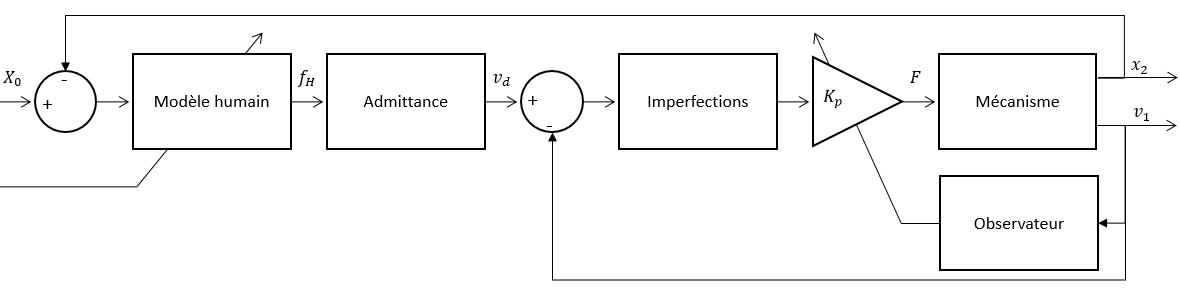
\includegraphics[width=14cm]{./img/cmd_meca_rob_hum.png}
    \caption{Commande des mécanisme robotique et humain}
    \label{fig:SchemaBlocComplet}
\end{figure}


\newpage
\section{Énoncé 2 : Simulation}
\subsection{Question 2.1}

\subsection{Question 2.2}

\subsection{Question 2.3}



\newpage
\section{Annexe}
\subsection{Annexe 1 : Liste des valeurs fixes}
\begin{itemize}
    \item[$$] \makebox[5cm][l]{\makebox[.6cm][l]{$M_R$} = 500 $kg$} \textit{(masse de la charge)}
    \item[$$] \makebox[5cm][l]{\makebox[.6cm][l]{$m_R$} = 50 $kg$} \textit{(masse du système)}
    \item[$$] \makebox[5cm][l]{\makebox[.6cm][l]{$K_B$} = 40000 $N/m$} \textit{(constante de raideur des courroies)}
    \item[$$] \makebox[5cm][l]{\makebox[.6cm][l]{$C_B$} = 40 $N\cdot s/m$} \textit{(coefficient d'amortissement des courroies)}
    \item[$$] \makebox[5cm][l]{\makebox[.6cm][l]{$C_H$} = 23.45 $N\cdot s/m$} \textit{(coefficient d'amortissement de l'humain)}
    \item[$$] \makebox[5cm][l]{\makebox[.6cm][l]{$C_R$} = 100 $N\cdot s/m$} \textit{(coefficient de frottement)}
    \item[$$] \makebox[5cm][l]{\makebox[.6cm][l]{$T$} = 0.1 $s$} \textit{(temps d'échantillonnage)}
\end{itemize}


\subsection{Lien vers le Dépôt GitHub}
\url{https://github.com/BlueWan14/Cours_IHR/tree/main/Devoir_2}

\end{document}
